%
% main.tex -- Paper zum Thema <lambertw>
%
% (c) 2020 Hochschule Rapperswil
%
\chapter{Verfolgungskurven\label{chapter:lambertw}}
\lhead{Verfolgungskurven}
\begin{refsection}
\chapterauthor{David Hugentobler und Yanik Kuster}
%
%Ein paar Hinweise für die korrekte Formatierung des Textes
%\begin{itemize}
%\item
%Absätze werden gebildet, indem man eine Leerzeile einfügt.
%Die Verwendung von \verb+\\+ ist nur in Tabellen und Arrays gestattet.
%\item
%Die explizite Platzierung von Bildern ist nicht erlaubt, entsprechende
%Optionen werden gelöscht. 
%Verwenden Sie Labels und Verweise, um auf Bilder hinzuweisen.
%\item
%Beginnen Sie jeden Satz auf einer neuen Zeile. 
%Damit ermöglichen Sie dem Versionsverwaltungssysteme, Änderungen
%in verschiedenen Sätzen von verschiedenen Autoren ohne Konflikt 
%anzuwenden.
%\item 
%Bilden Sie auch für Formeln kurze Zeilen, einerseits der besseren
%Übersicht wegen, aber auch um GIT die Arbeit zu erleichtern.
%\end{itemize}
%
%
% einleitung.tex -- Beispiel-File für die Einleitung
%
% (c) 2020 Prof Dr Andreas Müller, Hochschule Rapperswil
%
\section{Teil 0\label{fresnel:section:teil0}}
\rhead{Teil 0}
Lorem ipsum dolor sit amet, consetetur sadipscing elitr, sed diam
nonumy eirmod tempor invidunt ut labore et dolore magna aliquyam
erat, sed diam voluptua \cite{fresnel:bibtex}.
At vero eos et accusam et justo duo dolores et ea rebum.
Stet clita kasd gubergren, no sea takimata sanctus est Lorem ipsum
dolor sit amet.

Lorem ipsum dolor sit amet, consetetur sadipscing elitr, sed diam
nonumy eirmod tempor invidunt ut labore et dolore magna aliquyam
erat, sed diam voluptua.
At vero eos et accusam et justo duo dolores et ea rebum.  Stet clita
kasd gubergren, no sea takimata sanctus est Lorem ipsum dolor sit
amet.



%%
% teil2.tex -- Umsetzung in C Programmen
%
% (c) 2022 Fabian Dünki, Hochschule Rapperswil
%
\section{Umsetzung
\label{0f1:section:teil2}}
\rhead{Umsetzung}
Zur Umsetzung wurden drei verschiedene Ansätze gewählt, die in
vollständiger Form auf Github \cite{0f1:code} zu finden sind.
Dabei wurde der Schwerpunkt auf die Funktionalität und eine gute
Lesbarkeit des Codes gelegt.
Die Unterprogramme wurde jeweils, wie die GNU Scientific Library,
\index{GNU Scientific Library}%
in C geschrieben.
Die Zwischenresultate wurden vom Hauptprogramm
in einem CSV-File gespeichert.
\index{CSV}%
Anschliessen wurde mit der Matplot-Library
\index{Matplot-Library}%
\index{Python}%
in Python die Resultate geplottet.

\subsection{Potenzreihe
\label{0f1:subsection:potenzreihe}}
Die naheliegendste Lösung ist die Programmierung der Potenzreihe
\begin{align}
    \label{0f1:umsetzung:0f1:eq}
    \mathstrut_0F_1(;c;z)
    &=
    \sum_{k=0}^\infty
    \frac{z^k}{(c)_k \cdot k!}
    &= 
    \frac{1}{c}
    +\frac{z^1}{(c+1) \cdot 1}
    + \cdots
    + \frac{z^{20}}{c(c+1)(c+2)\cdots(c+19) \cdot 2.4 \cdot 10^{18}}.
\end{align}

\lstinputlisting[style=C,float,caption={Potenzreihe.},label={0f1:listing:potenzreihe}, firstline=59]{papers/0f1/listings/potenzreihe.c}

\subsection{Kettenbruch
\label{0f1:subsection:kettenbruch}}
Eine weitere Variante zur Berechnung von $\mathstrut_0F_1(;c;z)$ ist die Umsetzung als Kettenbruch.
\index{Kettenbruch}
Der Vorteil einer Umsetzung als Kettenbruch gegenüber der Potenzreihe ist die schnellere Konvergenz.

\subsubsection{Grundlage}
Ein endlicher Kettenbruch \cite{0f1:wiki-kettenbruch} ist ein Bruch der Form
\begin{equation*}
a_0 + \cfrac{b_1}{a_1+\cfrac{b_2}{a_2+\cfrac{b_3}{a_3+\cdots}}},
\end{equation*}
in welchem $a_0, a_1,\dots,a_n$ und $b_1,b_2,\dots,b_n$ ganze Zahlen sind.

\subsubsection{Rekursionsbeziehungen und Kettenbrüche}

Nimmt man die Gleichung
Wenn es für die analytischen Funktionen $f_i(z)$ eine Relation der Form
\begin{equation}
	f_{i-1}(z) - f_i(z) = k_i z f_{i+1}(z)
\label{0f1:relation}
\end{equation}
für ganzzahlige positive $i$ und Konstanten $k_i$
gibt,
dann gibt es einen Kettenbruch für das Verhältnis
$\frac{f_i(z)}{f_{i-1}(z)}$ \cite{0f1:wiki-fraction}. 
Aus der Relation~\eqref{0f1:relation}
ergibt sich der Zusammenhang
\begin{equation}
	\cfrac{f_i(z)}{f_{i-1}(z)}
	=
	\cfrac{1}{1+k_iz\cfrac{f_{i+1}(z)}{f_i(z)}}.
\label{0f1:bruchrelation}
\end{equation}
Geht man einen Schritt weiter und nimmt für
$g_i(z) = \frac{f_i(z)}{f_{i-1}(z)}$ an, kommt man zur Formel
\begin{equation*}
	g_i(z) = \cfrac{1}{1+k_izg_{i+1}(z)}.
\end{equation*}
Setzt man dies nun für $g_1$ in den Bruch ein, ergibt sich
\begin{equation*}
	g_1(z) = \cfrac{f_1(z)}{f_0(z)} = \cfrac{1}{1+k_izg_2(z)} = \cfrac{1}{1+\cfrac{k_1z}{1+k_2zg_3(z)}} = \cdots
\end{equation*}
Wiederholt man dies unendlich, erhält man einen Kettenbruch in der Form:
\begin{equation}
	\label{0f1:math:rekursion:eq}
	\cfrac{f_1(z)}{f_0(z)}
	=
	\cfrac{1}{1+\cfrac{k_1z}{1+\cfrac{k_2z}{1+\cfrac{k_3z}{\cdots}}}}.
\end{equation}

\subsubsection{Rekursion für $\mathstrut_0F_1$}
Angewendet auf die Potenzreihe
\begin{equation}
	\label{0f1:math:potenzreihe:0f1:eq}
	\mathstrut_0F_1(;c;z)
	=
	1 + \frac{z}{c\cdot1!} + \frac{z^2}{c(c+1)\cdot2!} + \frac{z^3}{c(c+1)(c+2)\cdot3!} + \cdots
\end{equation}
kann durch Substitution bewiesen werden, dass
\begin{equation*}
	\mathstrut_0F_1(;c-1;z) - \mathstrut_0F_1(;c;z)
	=
	\frac{z}{c(c-1)} \cdot \mathstrut_0F_1(;c+1;z)
\end{equation*}
eine Relation der Art \eqref{0f1:relation} dazu ist.
Wenn man für $f_i$ und $k_i$ die Annahme
\begin{align*}
	f_i &= \mathstrut_0F_1(;c+i;z)\\
	k_i	&= \frac{1}{(c+i)(c+i-1)}
\end{align*}
trifft und in die Formel \eqref{0f1:math:rekursion:eq} einsetzt, erhält man:
\begin{equation*}
	\cfrac{\mathstrut_0F_1(;c+1;z)}{\mathstrut_0F_1(;c;z)}
	=
	\cfrac{1}{1+\cfrac{\cfrac{z}{c(c+1)}}{1+\cfrac{\cfrac{z}{(c+1)(c+2)}}{1+\cfrac{\cfrac{z}{(c+2)(c+3)}}{\cdots}}}}.
\end{equation*}

\subsubsection{Algorithmus}
Da mit obigen Formeln nur ein Verhältnis zwischen
$\frac{\mathstrut_0F_1(;c+1;z)}{\mathstrut_0F_1(;c;z)}$
berechnet wurde, braucht es weitere Relationen um $\mathstrut_0F_1(;c;z)$
zu erhalten.
So ergeben ähnliche Relationen nach Wolfram Alpha \cite{0f1:wolfram-0f1} den Kettenbruch
\begin{equation}
	\label{0f1:math:kettenbruch:0f1:eq}
	\mathstrut_0F_1(;c;z) = 1 + \cfrac{\cfrac{z}{c}}{1+\cfrac{-\cfrac{z}{2(c+1)}}{1+\cfrac{z}{2(c+1)}+\cfrac{-\cfrac{z}{3(c+2)}}{1+\cfrac{z}{5(c+4)} + \cdots}}},
\end{equation}
der als Code (Listing \ref{0f1:listing:kettenbruchIterativ})  umgesetzt wurde. 

\lstinputlisting[style=C,float,caption={Iterativ umgesetzter Kettenbruch.},label={0f1:listing:kettenbruchIterativ},  firstline=8]{papers/0f1/listings/kettenbruchIterativ.c}

\subsection{Rekursionsformel
\label{0f1:subsection:rekursionsformel}}
Wesentlich stabiler zur Berechnung eines Kettenbruches ist die
Rekursionsformel.
\index{Rekursionsformel}%
Nachfolgend wird die verkürzte Herleitung vom
Kettenbruch zur Rekursionsformel aufgezeigt.
Eine vollständige Schritt für Schritt Herleitung ist im Seminarbuch Numerik
\cite{0f1:kettenbrueche}
im Kapitel Kettenbrüche zu finden.

\subsubsection{Herleitung}
Ein Näherungsbruch in der Form
\index{Näherungsbruch}%
\begin{align*}
	\cfrac{A_k}{B_k} = a_k + \cfrac{b_{k + 1}}{a_{k + 1} + \cfrac{p}{q}}
\end{align*}
lässt sich zu
\begin{align*}
	\cfrac{A_k}{B_k} = \cfrac{b_{k+1}}{a_{k+1} + \cfrac{p}{q}} = \frac{b_{k+1} \cdot q}{a_{k+1} \cdot q + p}
\end{align*}
umformen.
Dies lässt sich auch durch die Matrizenschreibweise
\index{Matrixschreibeweise eines Kettenbruchs}%
\begin{equation*}
	\begin{pmatrix}
		A_k\\
		B_k
	\end{pmatrix}
	= 		\begin{pmatrix}
		b_{k+1} \cdot q\\
		a_{k+1} \cdot q + p
	\end{pmatrix}
	=\begin{pmatrix}
		0&	b_{k+1}\\
		1&	a_{k+1}
	\end{pmatrix}
	\begin{pmatrix}
		p \\
		q
	\end{pmatrix}
	%\label{0f1:math:rekursionsformel:herleitung}
\end{equation*}
ausdrücken.
Wendet man dies nun auf den Kettenbruch in der Form
\begin{equation*}
	\frac{A_k}{B_k} = a_0 + \cfrac{b_1}{a_1+\cfrac{b_2}{a_2+\cfrac{\cdots}{\cdots+\cfrac{b_{k-1}}{a_{k-1} + \cfrac{b_k}{a_k}}}}}
\end{equation*}
an, ergibt sich die Matrixdarstellungen:
\begin{align*}
	\begin{pmatrix}
		A_k\\
		B_k
	\end{pmatrix}
	&=
	\begin{pmatrix}
		1& a_0\\
		0& 1
	\end{pmatrix}
	\begin{pmatrix}
		0& b_1\\
		1& a_1
	\end{pmatrix}
	\cdots
	\begin{pmatrix}
		0& b_{k-1}\\
		1& a_{k-1}
	\end{pmatrix}
	\begin{pmatrix}
		b_k\\
		a_k
	\end{pmatrix}.
\end{align*}
Nach vollständiger Induktion ergibt sich für den Schritt $k$, die Matrix
\begin{equation}
	\label{0f1:math:matrix:ende:eq}
	 \begin{pmatrix}
		A_{k}\\
		B_{k}			
	\end{pmatrix} 
	=
		\begin{pmatrix}
		A_{k-2}& A_{k-1}\\
		B_{k-2}& B_{k-1}			
	\end{pmatrix}
		\begin{pmatrix}
		b_k\\
		a_k
	\end{pmatrix}.
\end{equation}
Und schlussendlich kann der Näherungsbruch
\[
\frac{A_k}{B_k}
\] 
berechnet werden.

\subsubsection{Algorithmus}
Die Berechnung von $A_k, B_k$ gemäss \eqref{0f1:math:matrix:ende:eq} kann man auch ohne die Matrizenschreibweise \cite{0f1:kettenbrueche} aufschreiben:
\begin{itemize}
\item Startbedingungen:
\begin{align*}
A_{-1} &= 0		&		A_0 &= a_0 \\
B_{-1} &= 1		&		B_0 &= 1 
\end{align*}
\item Schritt $k\to k+1$:
\[
\begin{aligned}
\label{0f1:math:loesung:eq}
A_{k+1} &= A_{k-1} \cdot b_k + A_k \cdot a_k \\
B_{k+1} &= B_{k-1} \cdot b_k + B_k \cdot a_k
\end{aligned}
\]
\item
Näherungsbruch: \qquad$\displaystyle\frac{A_k}{B_k}$.
\end{itemize}
Ein grosser Vorteil dieser Umsetzung
als Rekursionsformel
(Listing~\ref{0f1:listing:kettenbruchRekursion}) ist,
dass im Vergleich zum Code (Listing~\ref{0f1:listing:kettenbruchIterativ})
eine Division gespart werden kann und somit weniger Rundungsfehler
entstehen können.

%Code
\lstinputlisting[style=C,float,caption={Rekursionsformel für Kettenbruch.},label={0f1:listing:kettenbruchRekursion},  firstline=8]{papers/0f1/listings/kettenbruchRekursion.c}

%%
% teil3.tex -- Beispiel-File für Teil 3
%
% (c) 2020 Prof Dr Andreas Müller, Hochschule Rapperswil
%
\section{Eigenschaften
\label{parzyl:section:Eigenschaften}}
\rhead{Eigenschaften}

\subsection{Potenzreihenentwicklung
	\label{parzyl:potenz}}
Die parabolischen Zylinderfunktionen, welche in Gleichung \ref{parzyl:eq:solution_dgl} gegeben sind, können auch als Potenzreihen geschrieben werden
\begin{align}
	w_1(k,z)
	&=  
	e^{-z^2/4} \,
	{}_{1} F_{1}
	(
	{\textstyle \frac{1}{4}} 
	- k, {\textstyle \frac{1}{2}} ; {\textstyle \frac{1}{2}}z^2) 
	= 
	e^{-\frac{z^2}{4}}
	\sum^{\infty}_{n=0}
	\frac{\left ( \frac{1}{4} - k \right )_{n}}{\left ( \frac{1}{2}\right )_{n}}
	\frac{\left ( \frac{1}{2} z^2\right )^n}{n!} \\
	&=
	e^{-\frac{z^2}{4}}
	\left ( 
	1 
	+
	\left ( \frac{1}{2} - 2k \right )\frac{z^2}{2!}
	+
	\left ( \frac{1}{2} - 2k \right )\left ( \frac{5}{2} - 2k \right )\frac{z^4}{4!}  
	+
	\dots
	\right )
\end{align}
und
\begin{align}
	w_2(k,z)
	&=  
	ze^{-z^2/4} \,
	{}_{1} F_{1}
	(
	{\textstyle \frac{3}{4}} 
	- k, {\textstyle \frac{3}{2}} ; {\textstyle \frac{1}{2}}z^2) 
	= 
	ze^{-\frac{z^2}{4}}
	\sum^{\infty}_{n=0}
	\frac{\left ( \frac{3}{4} - k \right )_{n}}{\left ( \frac{3}{2}\right )_{n}}
	\frac{\left ( \frac{1}{2} z^2\right )^n}{n!} \\
	&=
	e^{-\frac{z^2}{4}}
	\left ( 
	z 
	+
	\left ( \frac{3}{2} - 2k \right )\frac{z^3}{3!}
	+
	\left ( \frac{3}{2} - 2k \right )\left ( \frac{7}{2} - 2k \right )\frac{z^5}{5!}  
	+
	\dots
	\right ).
\end{align}
Bei den Potenzreihen sieht man gut, dass die Ordnung des Polynoms im generellen ins unendliche geht. Es gibt allerdings die Möglichkeit für bestimmte k das die Terme in der Klammer gleich null werden und das Polynom somit eine endliche Ordnung $n$ hat. Dies geschieht bei $w_1(k,z)$ falls
\begin{equation}
	k = \frac{1}{4} + n \qquad n \in \mathbb{N}_0
\end{equation}
und bei $w_2(k,z)$ falls
\begin{equation}
	k = \frac{3}{4} + n \qquad n \in \mathbb{N}_0.
\end{equation}

\subsection{Ableitung}
Es kann gezeigt werden, dass die Ableitungen $\frac{\partial w_1(z,k)}{\partial z}$ und $\frac{\partial w_2(z,k)}{\partial z}$ einen Zusammenhang zwischen $w_1(z,k)$ und $w_2(z,k)$ zeigen. Die Ableitung von $w_1(z,k)$ nach $z$ kann über die Produktregel berechnet werden und ist gegeben als
\begin{equation}
	\frac{\partial w_1(z,k)}{\partial z} = \left (\frac{1}{2} - 2k \right ) w_2(z, k -\frac{1}{2}) - \frac{1}{2} z w_1(z,k),
\end{equation} 
und die Ableitung von $w_2(z,k)$ als
\begin{equation}
	\frac{\partial w_2(z,k)}{\partial z} = w_1(z, k -\frac{1}{2}) - \frac{1}{2} z w_2(z,k).
\end{equation}
Über diese Eigenschaft können einfach weitere Ableitungen berechnet werden. 


%
% teil3.tex -- Beispiel-File für Teil 3
%
% (c) 2020 Prof Dr Andreas Müller, Hochschule Rapperswil
%
\section{Beispiel einer Verfolgungskurve
\label{lambertw:section:teil4}}
\rhead{Beispiel einer Verfolgungskurve}
In diesem Abschnitt wird rechnerisch das Beispiel einer Verfolgungskurve mit der Verfolgungsstrategie ``Jagd'' beschrieben. Dafür werden zuerst Bewegungsraum, Anfangspositionen und Bewegungsverhalten definiert, in einem nächsten Schritt soll eine Differentialgleichung dafür aufgestellt und anschliessend gelöst werden.

\subsection{Anfangsbedingungen definieren und einsetzen
	\label{lambertw:subsection:Anfangsbedingungen}}
Das zu verfolgende Ziel \(Z\) bewegt sich entlang der \(y\)-Achse mit konstanter Geschwindigkeit \(|\dot{z}| = 1\), beginnend beim Ursprung des kartesischen Koordinatensystems. Der Verfolger \(V\) startet auf einem beliebigen Punkt im ersten Quadranten und bewegt sich auch mit konstanter Geschwindigkeit \(|\dot{v}| = 1\) in Richtung Ziel. Aus diesen Bedingungen ergibt sich den ersten Quadranten als Bewegungsraum für \(V\). Diese Anfangspunkte oder Anfangsbedingungen können wie folgt formuliert werden:
\begin{equation}
	Z
	=
	\left( \begin{array}{c} 0 \\ |\dot{z}| \cdot t \end{array} \right)
	=
	\left( \begin{array}{c} 0 \\ t \end{array} \right)
	,\:
	V
	=
	\left( \begin{array}{c} x \\ y \end{array} \right)
	\:\text{und}\:\:
	|\dot{v}|
	=
	1.
	\label{lambertw:Anfangsbed}
\end{equation}
Wir haben nun die Anfangsbedingungen definiert, jetzt fehlt nur noch eine DGL, welche die fortlaufende Änderung der Position und Bewegungsrichtung des Verfolgers beschreibt. 
Diese DGL haben wir bereits in Kapitel \ref{lambertw:subsection:Verfolger} definiert, und zwar Gleichung \eqref{lambertw:pursuerDGL}. Wenn man die Startpunkte einfügt, ergibt sich der Ausdruck
\begin{equation}
	\frac{\left( \begin{array}{c} 0-x \\ t-y \end{array} \right)}{\sqrt{x^2 + (t-y)^2}}
	\cdot
	\left(\begin{array}{c} \dot{x} \\ \dot{y} \end{array}\right)
	=
	1.
	\label{lambertw:eqMitAnfangsbed}
\end{equation}

\subsection{Differentialgleichung vereinfachen
	\label{lambertw:subsection:DGLvereinfach}}
Nun haben wir eine Gleichung, es stellt sich aber die Frage, ob es überhaupt eine geschlossene Lösung dafür gibt. Eine Funktion welche die Beziehung \(y(x)\) beschreibt oder sogar \(x(t)\) und \(y(t)\) liefert. Zum jetzigen Zeitpunkt mag es nicht trivial scheinen, aber mit den gewählten Anfangsbedingungen \eqref{lambertw:Anfangsbed} ist es möglich, eine geschlossene Lösung für die Gleichung \eqref{lambertw:eqMitAnfangsbed} zu finden.

Auf dem Weg dahin muss die definierte DGL zuerst wesentlich vereinfacht werden, sei es mittels algebraischer Umformungen oder mit den Tools aus der Analysis. Da die nächsten Schritte sehr algebralastig sind und sie das Lesen dieses Papers träge machen würden, werden wir uns hier nur auf die wesentlichsten Schritte konzentrieren, welche notwendig sind, um den Lösungsweg nachvollziehen zu können.

\subsubsection{Skalarprodukt auflösen
	\label{lambertw:subsubsection:SkalProdAufl}}
Zuerst müssen wir den Bruch und das Skalarprodukt in \eqref{lambertw:eqMitAnfangsbed} wegbringen, damit wir eine viel handlichere Differentialgleichung erhalten. Dies führt zu
\begin{equation}
		-x \cdot \dot{x} + (t-y) \cdot \dot{y}
		= \sqrt{x^2 + (t-y)^2}.
		\label{lambertw:eqOhneSkalarprod}
\end{equation}
Im letzten Schritt, fällt die Nützlichkeit des Skalarproduktes in der Verfolgungsgleichung \eqref{lambertw:pursuerDGL} markant auf. Anstatt zwei gekoppelte Differentialgleichungen zu erhalten, eine für die \(x\)- und die andere für die \(y\)-Komponente, erhält man einen einzigen Ausdruck, was in der Regel mit weniger Lösungsaufwand verbunden ist.

\subsubsection{Quadrieren und Gruppieren
	\label{lambertw:subsubsection:QuadUndGrup}}
Mit der Quadratwurzel in \eqref{lambertw:eqOhneSkalarprod} kann man nichts anfangen, sie steht nur im Weg, also muss man sie loswerden. Wenn man dies macht, kann \eqref{lambertw:eqOhneSkalarprod} auf die Form  
\begin{equation}
	\left(\dot{x}^2-1\right) \cdot x^2 -2x \left(t-y\right) \dot{x}\dot{y} + \left(\dot{y}^2-1\right) \cdot \left(t-y\right)^2
	=0
	\label{lambertw:eqOhneWurzel}
\end{equation}
gebracht werden.
Diese Form mag auf den ersten Blick nicht gerade nützlich sein, aber man kann sie mit einer Substitution weiter vereinfachen.

\subsubsection{Wichtige Substitution
	\label{lambertw:subsubsection:WichtSubst}}
Wenn man beachtet, dass die Geschwindigkeit des Verfolgers konstant und gleich 1 ist, dann ergibt sich die Beziehung  
\begin{equation}
	\dot{x}^2 + \dot{y}^2 
	= 1.
	\label{lambertw:eqGeschwSubst}
\end{equation}
Umformungen der Gleichung \eqref{lambertw:eqGeschwSubst} können in \eqref{lambertw:eqOhneWurzel} erkannt werden. Wenn man sie ersetzt, erhält man
\begin{equation}
		\dot{y}^2 \cdot x^2 +2x \left(t-y\right) \dot{x}\dot{y} + \dot{x}^2 \cdot \left(t-y\right)^2
		=0.
		\label{lambertw:eqGeschwSubstituiert}
\end{equation}
Diese unscheinbare Substitution führt dazu, dass weitere Vereinfachungen durchgeführt werden können.

\subsubsection{Binom erkennen und vereinfachen
	\label{lambertw:subsubsection:BinomVereinfach}}
Versteckt im Ausdruck \eqref{lambertw:eqGeschwSubstituiert} befindet sich die erste binomische Formel, wobei
\begin{equation}
	(x \dot{y} + (t-y) \dot{x})^2
	= 0
	\label{lambertw:eqAlgVerinfacht}
\end{equation}
die faktorisierte Darstellung davon ist.
Da der linke Term gleich Null ist, muss auch die Basis des Quadrates in \eqref{lambertw:eqAlgVerinfacht} gleich Null sein. Es ergibt sich eine weitere Vereinfachung, welche zu der im Vergleich zu \eqref{lambertw:eqOhneSkalarprod} wesentlich einfacheren DGL 
\begin{equation}
	x \dot{y} + (t-y) \dot{x}
	= 0
	\label{lambertw:eqGanzVerinfacht}
\end{equation}
führt.
Kompakt, ohne Wurzelterme und Quadrate, nur elementare Operationen und Ableitungen. 

Nun stellt sich die Frage wie es weiter gehen soll, bei der Gleichung \eqref{lambertw:eqGanzVerinfacht} scheinen keine weiteren Vereinfachungen möglich zu sein. Wir brauchen einen neuen Ansatz, um unser Ziel einer möglichen Lösung zu verfolgen.

\subsection{Zeitabhängigkeit loswerden
	\label{lambertw:subsection:ZeitabhLoswerden}}
Der nächste logische Schritt scheint irgendwie die Zeitabhängigkeit in der Gleichung \eqref{lambertw:eqGanzVerinfacht} loszuwerden, aber wieso? Nun, wie am Anfang von Abschnitt \ref{lambertw:subsection:DGLvereinfach} beschrieben, suchen wir eine Lösung der Art \(y(x)\), dies ist natürlich erst möglich wenn wir die Abhängigkeit nach \(t\) eliminieren können.

\subsubsection{Zeitliche Ableitungen loswerden
	\label{lambertw:subsubsection:ZeitAbleit}}
Der erste Schritt auf dem Weg zur Funktion \(y(x)\) ist, die zeitlichen Ableitungen los zu werden, dafür wird \eqref{lambertw:eqGanzVerinfacht} beidseitig durch \(\dot{x}\) dividiert, was erlaubt ist, weil diese Änderung ungleich Null ist:
\begin{equation}
	x \frac{\dot{y}}{\dot{x}} + (t-y) \frac{\dot{x}}{\dot{x}}
	= 0.
	\label{lambertw:eqVorKeineZeitAbleit}
\end{equation}
Der Grund dafür ist, dass
\begin{equation}
	\frac{\displaystyle\dot{y}}{\displaystyle\dot{x}} 
	= \frac{\displaystyle\frac{dy}{dt}}{\displaystyle\frac{dx}{dt}}  
	= \frac{dy}{dx}
	= y^{\prime},
	\label{lambertw:eqQuotZeitAbleit}
\end{equation}
und somit kann der Quotient dieser zeitlichen Ableitungen in eine Ableitung nach \(x\) umgewandelt werden.
Nachdem die Eigenschaft \eqref{lambertw:eqQuotZeitAbleit} in \eqref{lambertw:eqVorKeineZeitAbleit} eingesetzt wurde, entsteht beim Vereinfachen die neue Gleichung
\begin{equation}
	x y^{\prime} + t - y
	= 0.
	\label{lambertw:DGLmitT}
\end{equation}

\subsubsection{Variable \(t\) eliminieren
	\label{lambertw:subsubsection:VarTelimin}}
Hier wäre es natürlich passend, wenn man die Abhängigkeit nach \(t\) komplett wegbringen könnte, aber wie?
Wir wissen, dass sich der Verfolger mit Geschwindigkeit 1 bewegt, also legt er in der Zeit \(t\) die Strecke \(1\cdot t = t\) zurück. Längen und Strecken können auch mit der Bogenlänge repräsentiert werden, somit kann Zeit und zurückgelegte Strecke in der Gleichung  
\begin{equation}
	s
	= 
	|\dot{v}| \cdot t
	=
	1 \cdot t
	=
	t
	=
	\int_{\displaystyle x_0}^{\displaystyle x_{\text{end}}}\sqrt{1+y^{\prime\, 2}} \: dx
	\label{lambertw:eqZuBogenlaenge}
\end{equation}
verbunden werden.
  
Nicht gerade auffällig ist die Richtung, in welche hier integriert wird. Wenn der Verfolger sich wie vorgesehen am Anfang im ersten Quadranten befindet, dann muss sich dieser nach links bewegen, was nicht der üblichen Integrationsrichtung entspricht. Um eine Integration wie üblich von links nach rechts ausführen zu können, müssen die Integrationsgrenzen vertauscht werden, was in einem Vorzeichenwechsel resultiert. 

Wenn man nun \eqref{lambertw:eqZuBogenlaenge} in die DGL \eqref{lambertw:DGLmitT} einfügt, dann ergibt sich der neue Ausdruck
\begin{equation}
	x y^{\prime} - \int\sqrt{1+y^{\prime\, 2}} \: dx - y
	= 0.
	\label{lambertw:DGLohneT}
\end{equation}
Um das Integral los zu werden, leitet man \eqref{lambertw:DGLohneT} nach \(x\) ab und erhält die DGL zweiter Ordnung 
\begin{align}
	y^{\prime}+ xy^{\prime\prime} - \sqrt{1+y^{\prime\, 2}} - y^{\prime}
	&= 0, \\
	xy^{\prime\prime} - \sqrt{1+y^{\prime\, 2}}
	&= 0.
	\label{lambertw:DGLohneInt}
\end{align}
Nun sind wir unserem Ziel einen weiteren Schritt näher. Die Gleichung \eqref{lambertw:DGLohneInt} mag auf den ersten Blick nicht gerade einfach sein, aber im nächsten Abschnitt werden wir sehen, dass sie relativ einfach zu lösen ist.

\subsection{Differentialgleichung lösen
	\label{lambertw:subsection:DGLloes}}
Die Gleichung \eqref{lambertw:DGLohneInt} ist eine DGL zweiter Ordnung, in der \(y\) nicht vorkommt. Sie kann mittels der Substitution \(y^{\prime} = u\) in die DGL
\begin{equation}
	xu^{\prime} - \sqrt{1+u^2}
	= 0
	\label{lambertw:DGLmitU}
\end{equation}
erster Ordnung umgewandelt werden.
Diese Gleichung ist separierbar, was sie viel handlicher macht. In der separierten Form
\begin{equation}
	\int{\frac{1}{\sqrt{1+u^2}}\:du} 
	= 
	\int{\frac{1}{x}\:dx},
\end{equation}
lässt sich die Gleichung mittels einer Integrationstabelle sehr rasch lösen. 
Das Ergebnis ist 
\begin{align}
	\operatorname{arsinh}(u)
	&=
	\operatorname{ln}(x) + C, \\
	u
	&=
	\operatorname{sinh}(\operatorname{ln}(x) + C).
	\label{lambertw:loesDGLmitU}
\end{align}
Wenn man in \eqref{lambertw:loesDGLmitU} die Substitution rückgängig macht, erhält man die DGL 
\begin{equation}
	y^{\prime}
	=
	\operatorname{sinh}(\operatorname{ln}(x) + C)
	\label{lambertw:loesDGLmitY}
\end{equation}
erster Ordnung, die bereits separiert ist.
Ersetzt man den \(\operatorname{sinh}\) durch seine exponentielle Definition \(\operatorname{sinh}(x)=\frac{1}{2}(e^x-e^{-x})\), so resultiert auf sehr einfache Art die Lösung 
\begin{equation}
	y
	=
	C_1 + C_2 x^2 - \frac{\operatorname{ln}(x)}{8 \cdot C_2}
\end{equation}
für \eqref{lambertw:loesDGLmitY}.

Nun haben wir eine Lösung, aber wie es immer mit Lösungen ist, stellt sich die Frage, ob sie überhaupt plausibel ist.

\subsection{Lösung analysieren
	\label{lambertw:subsection:LoesAnalys}}

\definecolor{applegreen}{rgb}{0.55, 0.71, 0.0}

\begin{figure}
	\centering
	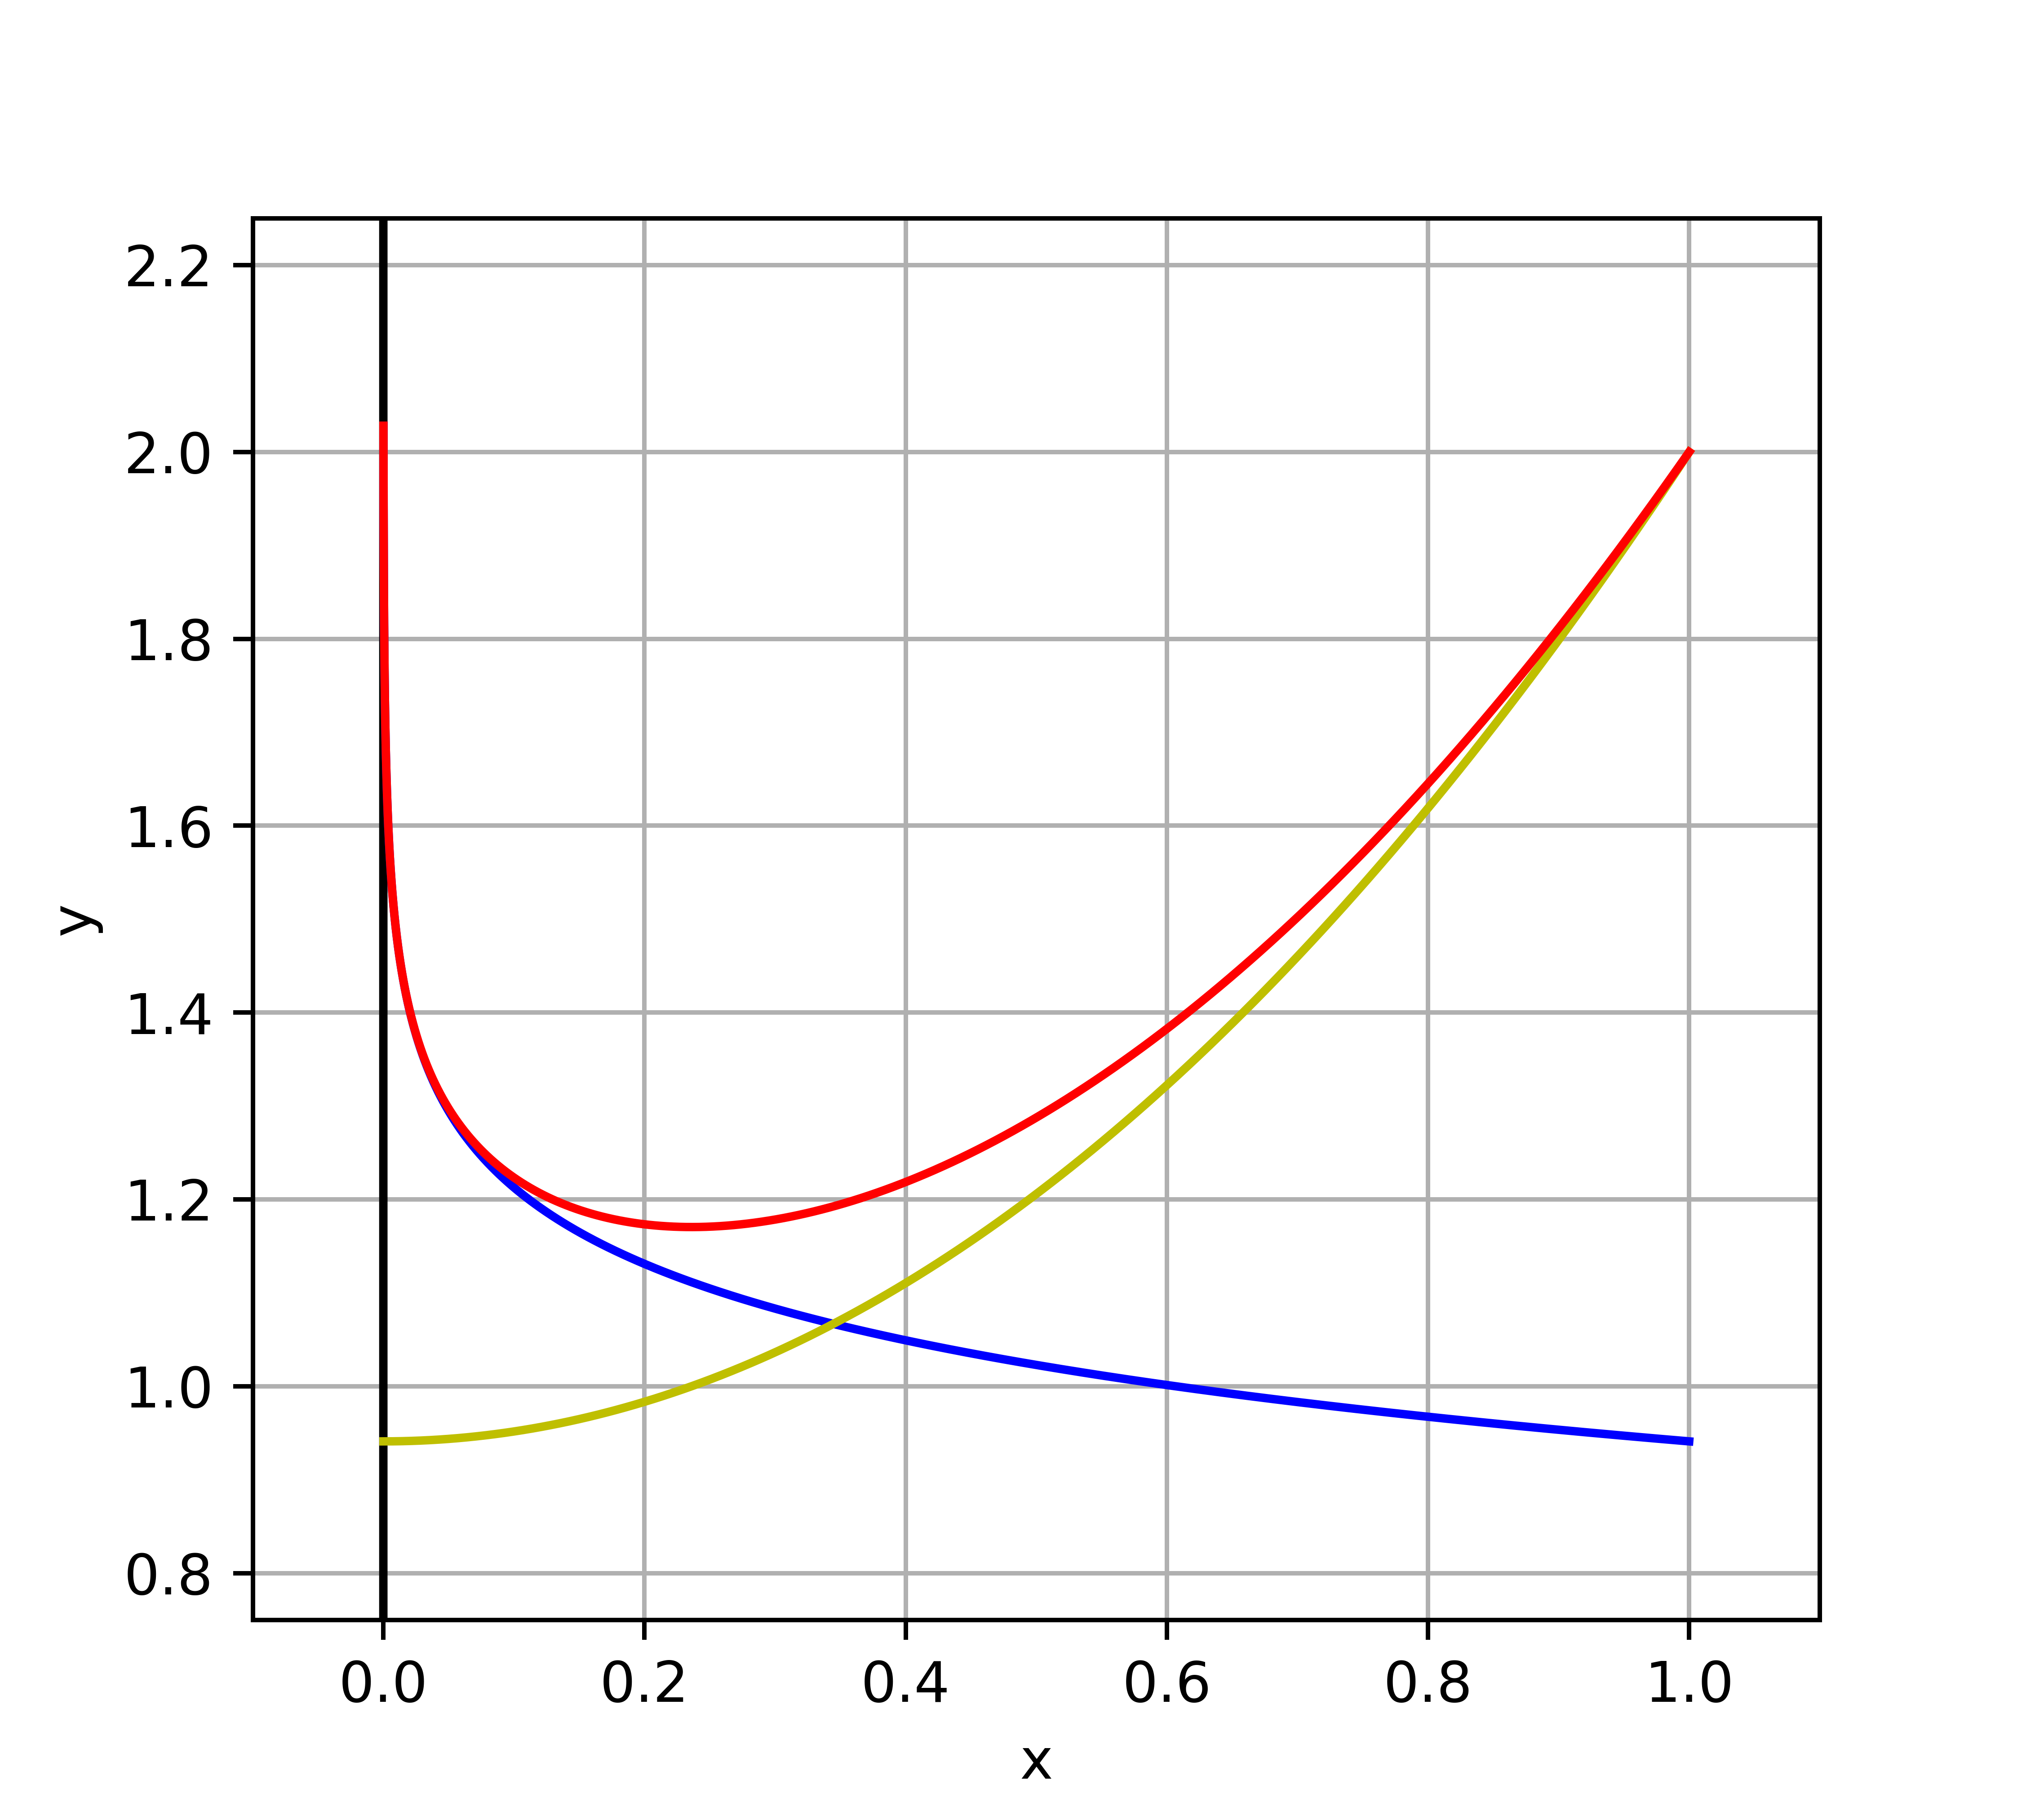
\includegraphics{papers/lambertw/Bilder/VerfolgungskurveBsp.png}
	\caption[Graph der Verfolgungskurve]{Graph der Verfolgungskurve wobei, ({\color{red}rot}) die Funktion \ensuremath{y(x)} ist, ({\color{applegreen}grün}) der quadratische Teil und ({\color{blue}blau}) dem \ensuremath{\operatorname{ln}(x)}-Teil entspricht.
	\label{lambertw:BildFunkLoes}
	}
\end{figure}

Das Resultat, wie ersichtlich, ist die Funktion  
\begin{equation}
	{\color{red}{y(x)}}
	=
	C_1 + C_2 {\color{applegreen}{x^2}} {\color{blue}{-}} \frac{\color{blue}{\operatorname{ln}(x)}}{8 \cdot C_2},
	\label{lambertw:funkLoes}
\end{equation}
für welche die Koeffizienten \(C_1\) und \(C_2\) aus den Anfangsbedingungen bestimmt werden können. Zuerst soll aber eine qualitative Intuition oder Idee für das Aussehen der Funktion \(y(x)\) geschaffen werden:
\begin{itemize}
	\item
	Für grosse \(x\)-Werte, welche in der Regel in der Nähe von \(x_0\) sein sollten, ist der quadratisch Term in der Funktion \eqref{lambertw:funkLoes} dominant. 
	\item
	Für immer kleiner werdende \(x\) geht der Verfolger in Richtung \(y\)-Achse, wobei seine Steigung stetig sinkt, was Sinn macht wenn der Verfolgte entlang der \(y\)-Achse steigt. Irgendwann werden Verfolger und Ziel auf gleicher Höhe sein, also gleiche \(y\)- aber verschiedene \(x\)-Koordinate besitzen.
	In diesem Punkt findet ein Monotoniewechsel in der Kurve \eqref{lambertw:funkLoes} statt, was zu einem Minimum führt.
	\item
	Für \(x\)-Werte in der Nähe von \(0\) ist das asymptotische Verhalten des Logarithmus dominant, dies macht auch Sinn, da sich der Verfolgte auf der \(y\)-Achse bewegt und der Verfolger ihm nachgeht.
\end{itemize}
Alle diese Eigenschaften stimmen mit dem überein, was man von einer Kurve dieser Art erwarten würde, welche durch die Grafik \ref{lambertw:BildFunkLoes} repräsentiert wurde.

\subsection{Anfangswertproblem 
	\label{lambertw:subsection:AllgLoes}}
In diesem Abschnitt soll eine Parameterfunktion hergeleitet werden, bei der jeder beliebige Anfangspunkt im ersten Quadranten eingesetzt werden kann, ausser der Ursprung im Koordinatensystem. Diese Aufgabe ist ein Anfangswertproblem für \(y(x)\).

Das Lösen des Anfangswertproblems ist ein Problem aus der Analysis, auf welches hier nicht explizit eingegangen wird. Zur Vollständigkeit und Nachvollziehbarkeit, wird aber das Gleichungssystem präsentiert, welches notwendig ist, um das Anfangswertproblem zu lösen.

\subsubsection{Anfangswerte bestimmen
	\label{lambertw:subsubsection:Anfangswerte}}
Der erste Schritt auf dem Weg zur gesuchten Parameterfunktion ist, die Anfangswerte 
\begin{equation}
	y(x)\big \vert_{t=0}
	=
	y(x_0)
	= 
	y_0
	\label{lambertw:eq1Anfangswert}
\end{equation}
und
\begin{equation}
	\frac{dy}{dx}\bigg \vert_{t=0}
	=
	y^{\prime}(x_0)
	=
	\frac{y_0}{x_0}
	\label{lambertw:eq2Anfangswert}
\end{equation}
zu definieren.
Der zweite Anfangswert \eqref{lambertw:eq2Anfangswert} mag nicht grade offensichtlich sein. Die Erklärung dafür ist aber simpel: Der Verfolger wird sich zum Zeitpunkt \(t=0\) in Richtung Koordinatenursprung bewegen wollen, wo sich das Ziel befindet. Somit entsteht das Steigungsdreieck mit \(\Delta x = x_0\) und \(\Delta y = y_0\).

\subsubsection{Gleichungssystem aufstellen und lösen
	\label{lambertw:subsubsection:GlSys}}
Wenn man die Anfangswerte \eqref{lambertw:eq1Anfangswert} und \eqref{lambertw:eq2Anfangswert} in die Gleichung \eqref{lambertw:funkLoes} und deren Ableitung \(y^{\prime}(x)\) einsetzt, dann ergibt sich das Gleichungssystem
\begin{subequations}
	\label{lambertw:eqGleichungssystem}
	\begin{align}
		y_0
		&=
		C_1 + C_2 x^2_0 - \frac{\operatorname{ln}(x_0)}{8 \cdot C_2}, \\
		\frac{y_0}{x_0}
		&=
		2 \cdot  C_2 x_0 - \frac{1}{8 \cdot C_2 \cdot x_0}.
	\end{align}
\end{subequations}
Damit die gesuchte Funktion im ersten Quadranten bleibt, werden nur die positiven Lösungen  
\begin{subequations}
	\begin{align}
		\label{lambertw:eqKoeff1}
		C_1
		&=
		\frac{2\cdot\operatorname{ln}(x_0)\left(\sqrt{x_0^2 + y_0^2} - y_0 \right) - \sqrt{x_0^2 + y_0^2} + 3 y_0}{4}, \\
		\label{lambertw:eqKoeff2}
		C_2
		&=
		\frac{\sqrt{x_0^2 + y_0^2} + y_0}{4x_0^2}
	\end{align}
\end{subequations}
des Gleichungssystems gewählt.
\subsubsection{Gesuchte Parameterfunktion aufstellen
	\label{lambertw:subsubsection:ParamFunk}}
Wenn man die Koeffizienten \eqref{lambertw:eqKoeff1} und \eqref{lambertw:eqKoeff2} in die Funktion \eqref{lambertw:funkLoes} einsetzt, dann ergibt sich beim Vereinfachen die gesuchte Parameterfunktion
\begin{equation}
	y(x)
	=
	\frac{1}{4}\left(\left(y_0+r_0\right)\eta+\left(y_0-r_0\right)
	\operatorname{ln}\left(\eta\right)-r_0+3y_0\right).
	\label{lambertw:eqAllgLoes}
\end{equation}
Damit die Funktion \eqref{lambertw:eqAllgLoes} trotzdem übersichtlich bleibt, wurden Anfangssteigung \(\eta\) und Anfangsentfernung \(r_0\) wie folgt definiert:
\begin{equation}
	\eta
	=
	\left(\frac{x}{x_0}\right)^2
	\:\:\text{und}\:\:
	r_0
	=
	\sqrt{x_0^2+y_0^2}.
\end{equation}
Diese neue allgemeine Funktion \eqref{lambertw:eqAllgLoes} weist immer noch die selbe Struktur wie die vorher hergeleitete Funktion \eqref{lambertw:funkLoes} auf. Sie enthält einerseits einen quadratischen Teil, der in \(\eta\) enthalten ist, anderseits den \(\operatorname{ln}\)-Teil. Aus dieser Ähnlichkeit kann geschlossen werden, dass sich \eqref{lambertw:eqAllgLoes} auf eine ähnliche Art verhalten wird.

Nun sind wir soweit, dass wir eine \(y(x)\)-Beziehung für beliebige Anfangswerte darstellen können, unser erstes Ziel wurde erreicht. Wir können aber einen Schritt weiter gehen und uns Fragen: Ist es analytisch möglich herauszufinden, wo sich Verfolger und Ziel zu jedem Zeitpunkt befinden? Dieser Frage werden wir im nächsten Abschnitt nachgehen.

\subsection{Funktion nach der Zeit 
	\label{lambertw:subsection:FunkNachT}}
In diesem Abschnitt werden algebraische Umformungen ein wenig detaillierter als zuvor beschrieben. Dies hat auch einen bestimmten Grund: Den Einsatz einer speziellen Funktion aufzeigen, sowie auch wann und wieso diese vorkommt. Welche spezielle Funktion? Fragt man sich wahrscheinlich in diesem Moment. Nun, um diese Frage kurz zu beantworten, es ist ``YouTube's favorite special function'' laut dem Mathematiker Michael Penn, die Lambert-\(W\)-Funktion \(W(x)\) welche im Kapitel \ref{buch:section:lambertw} bereits beschrieben wurde.

\subsubsection{Zeitabhängigkeit wiederherstellen
	\label{lambertw:subsubsection:ZeitabhWiederherst}}
Der erste Schritt ist es herauszufinden, wie die Zeitabhängigkeit wieder hineingebracht werden kann. Dafür greifen wir auf die letzte Gleichung zu, in welcher \(t\) noch enthalten war, und zwar DGL 
\begin{equation}
	x y^{\prime} + t - y
	= 0
	\label{lambertw:eqDGLmitTnochmals}
\end{equation}
aus dem Abschnitt \eqref{lambertw:subsection:ZeitabhLoswerden}, welche zur Übersichtlichkeit hier nochmals aufgeführt wurde.
Wie in \eqref{lambertw:eqDGLmitTnochmals} zu sehen ist, werden \(y\) und deren Ableitung \(y^{\prime}\) benötigt, diese sind:
\begin{subequations}
	\label{lambertw:eqFunkUndAbleit}
	\begin{align}
		\label{lambertw:eqFunkUndAbleit1}
		y
		&=
		\frac{1}{4}\left(\left(y_0+r_0\right)\eta+\left(y_0-r_0\right)\operatorname{ln}\left(\eta\right)-r_0+3y_0\right), \\
		y^\prime
		&=
		\frac{1}{2}\biggl(\left(y_0+r_0\right)\frac{x}{x_0^2}+\left(y_0-r_0\right)\frac{1}{x}\biggr).
	\end{align}
\end{subequations}

Wenn man diese Gleichungen \eqref{lambertw:eqFunkUndAbleit} in die DGL \eqref{lambertw:eqDGLmitTnochmals} einfügt, vereinfacht und nach \(t\) auflöst, dann ergibt sich der Ausdruck
\begin{equation}
	-4t
	=
	\left(y_0+r_0\right)\left(\eta-1\right)+\left(r_0-y_0\right)\operatorname{ln}\left(\eta\right).
	\label{lambertw:eqFunkUndAbleitEingefuegt}
\end{equation}

\subsubsection{Umformungen die zur Funktion nach der Zeit führen
	\label{lambertw:subsubsection:UmformBisZumZiel}}
Mit dem Ausdruck \eqref{lambertw:eqFunkUndAbleitEingefuegt}, welcher Terme mit \(x\) und \(t\) verbindet, kann nun nach der gesuchten Variable \(x\) aufgelöst werden. 

In einem nächsten Schritt wird alles mit \(x\) auf die eine Seite gebracht, der Rest auf die andere Seite und anschliessend beidseitig exponenziert, sodass man 
\begin{equation}
	-4t+\left(y_0+r_0\right)
	=
	\left(y_0+r_0\right)\eta+\left(r_0-y_0\right)\operatorname{ln}\left(\eta\right)
\end{equation}
und anschliessend
\begin{equation}
	e^{\displaystyle -4t+\left(y_0+r_0\right)}
	=
	e^{\displaystyle \left(y_0+r_0\right)\eta}\cdot\eta^{\displaystyle \left(r_0-y_0\right)}
	\label{lambertw:eqMitExp}
\end{equation}
erhält.
Auf dem rechten Term von \eqref{lambertw:eqMitExp} beginnen wir langsam eine ähnliche Struktur wie \(\eta e^\eta\) zu erkennen, dies schreit nach der Struktur, die benötigt wird, um \(\eta\) mittels der Lambert-\(W\)-Funktion \(W(x)\) zu erhalten. Dies macht durchaus Sinn, wenn wir die Funktion \(x(t)\) finden wollen und \(W(x)\) die Umkehrfunktion von \(x e^x\) ist. 

Die erste Sache, die uns in \eqref{lambertw:eqMitExp} stört ist, dass \(\eta\) als Potenz da steht. Dieses Problem können wir loswerden, indem wir beidseitig mit \(\:1 / (r_0-y_0)\:\) potenzieren:
\begin{equation}
	\operatorname{exp}\left(\displaystyle \frac{-4t}{r_0-y_0}+\frac{y_0+r_0}{r_0-y_0}\right)
	=
	\eta\cdot \operatorname{exp}\left(\displaystyle \frac{y_0+r_0}{r_0-y_0}\eta\right).
	\label{lambertw:eqOhnePotenz}
\end{equation}

\subsubsection{Eine essenzielle Substitution
	\label{lambertw:subsubsection:SubstChi}}
Das nächste Problem, auf welches wir in \eqref{lambertw:eqOhnePotenz} treffen, ist, dass \(\eta\) nicht alleine im Exponent steht. Dies kann elegant mit der Substitution 
\begin{equation}
	\chi
	=
	\frac{y_0+r_0}{r_0-y_0}
	\label{lambertw:eqChiSubst}
\end{equation}
gelöst werden.
Es gäbe natürlich andere Substitutionen wie z.B. 
\[\displaystyle \chi=\frac{y_0+r_0}{r_0-y_0}\cdot\eta,\] 
die auf dasselbe Ergebnis führen würden, aber \eqref{lambertw:eqChiSubst} liefert in einem Schritt die kompakteste Lösung. Also fahren wir mit der Substitution \eqref{lambertw:eqChiSubst} weiter, setzen diese in die Gleichung \eqref{lambertw:eqOhnePotenz} ein und multiplizieren beidseitig mit \(\chi\). Daraus erhalten wir die Gleichung
\begin{equation}
	\chi\cdot \operatorname{exp}\left(\displaystyle \chi-\frac{4t}{r_0-y_0}\right)
	=
	\chi\eta\cdot e^{\displaystyle \chi\eta}.
	\label{lambertw:eqNachSubst}
\end{equation}

\subsubsection{Funktion nach der Zeit dank Lambert-\(W\)
	\label{lambertw:subsubsection:LambertWundFvonT}}
Nun sind wir endlich soweit, dass wir die angedeutete Lambert-\(W\)-Funktion \(W(x)\) einsetzen können. Wenn wir beidseitig \(W(x)\) anwenden, dann erhalten wir den Ausdruck
\begin{equation}
	W\left(\chi\cdot \operatorname{exp}\left(\displaystyle \chi-\frac{4t}{r_0-y_0}\right)\right)
	=
	\chi\eta.
\end{equation}
Nach dem Auflösen nach \(x\) welches in \(\eta\) enthalten ist, erhalten wir die gesuchte \(x(t)\)-Funktion \eqref{lambertw:eqFunkXNachT}. Dieses \(x(t)\) in Kombination mit \eqref{lambertw:eqFunkUndAbleit1} liefert die Position des Verfolgers zu jedem Zeitpunkt. Das Gleichungspaar besteht also aus den Gleichungen
\begin{subequations}
	\label{lambertw:eqFunktionenNachT}
	\begin{align}
		\label{lambertw:eqFunkXNachT}
		x(t)
		&=
		x_0\cdot\sqrt{\frac{W\left(\chi\cdot \operatorname{exp}\left(\displaystyle \chi-\frac{4t}{r_0-y_0}\right)\right)}{\chi}}, \\
		\label{lambertw:eqFunkYNachT}
		y(x(t))
		=
		y(t)
		&=
		\frac{1}{4}\biggl(\left(y_0+r_0\right)\left(\frac{x(t)}{x_0}\right)^2+\left(y_0-r_0\right)\operatorname{ln}\biggl(\biggl(\frac{x(t)}{x_0}\biggr)^2\biggr)-r_0+3y_0\biggr).
	\end{align}
\end{subequations}
Nun haben wir unser letztes Ziel erreicht und sind in der Lage eine Verfolgung rechnerisch sowie graphisch zu repräsentieren.

\subsubsection{Hinweise zur Lambert-\(W\)-Funktion
	\label{lambertw:subsubsection:HinwLambertW}}
Wir sind aber noch nicht ganz fertig, eine Frage muss noch beantwortet werden. Und zwar wieso man schon bei der Gleichung \eqref{lambertw:eqFunkUndAbleitEingefuegt} weiss, dass die Lambert-\(W\)-Funktion zum Einsatz kommen wird.
Nun, der Grund dafür ist die Struktur
\begin{equation}
	y
	=
	p(x) +\operatorname{ln}(x),
	\label{lambertw:eqEinsatzLambW}
\end{equation}
bei welcher \(p(x)\) eine beliebige Potenz von \(x\) darstellt. 

Jedes Mal wenn \(x\) gesucht ist und in einer Struktur der Art \eqref{lambertw:eqEinsatzLambW} vorkommt, dann kann mit ein paar Umformungen die Struktur \(f(x)e^{f(x)}\) erzielt werden. Wie bereits in diesem Abschnitt \ref{lambertw:subsection:FunkNachT} gezeigt wurde, kann \(x\) nun mittels der \(W(x)\)-Funktion aufgelöst werden. Erstaunlicherweise ist \eqref{lambertw:eqEinsatzLambW} eine Struktur die oft vorkommt, was die Lambert-\(W\)-Funktion so wichtig macht.   
%
% teil1.tex -- Beispiel-File für das Paper
%
% (c) 2020 Prof Dr Andreas Müller, Hochschule Rapperswil
%
\section{Lösung
\label{parzyl:section:teil1}}
\rhead{Problemstellung}
Die Differentialgleichungen \eqref{parzyl:sep_dgl_1} und \eqref{parzyl:sep_dgl_2} können mit
Hilfe der Whittaker Gleichung gelöst werden.
\begin{definition}
    Die Funktion 
    \begin{equation*}
        W_{k,m}(z) = 
    e^{-z/2} z^{m+1/2} \,
    {}_{1} F_{1}
    (
        {\textstyle \frac{1}{2}} 
        + m - k, 1 + 2m; z)
    \end{equation*}
    heisst Whittaker Funktion und ist eine Lösung
    von der Whittaker Differentialgleichung
    \begin{equation}
        \frac{d^2W}{d z^2} +
        \left(-\frac{1}{4}  + \frac{k}{z} + \frac{\frac{1}{4} - m^2}{z^2} \right) W = 0.
        \label{parzyl:eq:whitDiffEq}
    \end{equation}
\end{definition}
Es wird nun die Differentialgleichung bestimmt, welche
\begin{equation}
    w = z^{-1/2} W_{k,-1/4} \left({\textstyle \frac{1}{2}} z^2\right)
\end{equation}
als Lösung hat.
Dafür wird $w$ in \eqref{parzyl:eq:whitDiffEq} eingesetzt woraus
\begin{equation}
    \frac{d^2 w}{dz^2} - \left(\frac{1}{4} z^2 - 2k\right) w = 0
\label{parzyl:eq:weberDiffEq}
\end{equation}
resultiert. DIese Differentialgleichung ist dieselbe wie 
\eqref{parzyl:sep_dgl_2} und \eqref{parzyl:sep_dgl_2}, welche somit
$w$ als Lösung haben.
Da es sich um eine Differentialgleichung zweiter Ordnung handelt, hat sie nicht nur
eine sondern zwei Lösungen.
Die zweite Lösung der Whittaker-Gleichung ist $W_{k,-m} (z)$.
Somit hat \eqref{parzyl:eq:weberDiffEq}
\begin{align}
    w_1 & = z^{-1/2} W_{k,-1/4} \left({\textstyle \frac{1}{2}} z^2\right)\\
    w_2 & = z^{-1/2} W_{k,1/4} \left({\textstyle \frac{1}{2}} z^2\right)
\end{align}
als Lösungen.

Ausgeschrieben ergeben sich als Lösungen
\begin{align}
    w_1 &= e^{-z^2/4} \,
    {}_{1} F_{1}
    (
        {\textstyle \frac{1}{4}} 
         - k, {\textstyle \frac{1}{2}} ; {\textstyle \frac{1}{2}}z^2) \\
    w_2 & = z e^{-z^2/4} \,
         {}_{1} F_{1}
         ({\textstyle \frac{3}{4}} 
              - k, {\textstyle \frac{3}{2}} ; {\textstyle \frac{1}{2}}z^2)
\end{align}
%
\printbibliography[heading=subbibliography]
\end{refsection}
